\documentclass{beamer}
\usepackage[T1]{fontenc}
\usepackage[utf8]{inputenc}
\usepackage{lmodern}
\usepackage{ngerman}
\usepackage{graphics}
\usepackage{amsmath}
\usepackage{algorithm}
\usepackage{algorithmicx}
\usetheme{Singapore}
\usecolortheme{dove}
\graphicspath{{images/}{../comics/}}
\newcommand{\hiddencell}[2]{\action<#1->{#2}}
\AtBeginSection[]
{
  \begin{frame}[plain]
    \frametitle{}
    {\footnotesize
      \tableofcontents[currentsection]
    }
  \end{frame}
}

\title{Grundbegriffe der Informatik}
\author{Patrick Niklaus}

\begin{document}
\begin{frame}
  \frametitle{Grundbegriffe der Informatik}
  \framesubtitle{2. Tutorium}
  \begin{description}
    \item \textbf{Name:} Patrick Niklaus
    \item \textbf{E-Mail:} patrick.niklaus@student.kit.edu
    \item \textbf{Nr:} 43
  \end{description}
\end{frame}

\section{Übungsblatt}
\begin{frame}
  \frametitle{Was oft falsch gemacht wurde:}
  \begin{itemize}
    \item ${\exists}_1$ oder $\exists !$ bitte nicht (in GBI) benutzen!\\
          ${\exists}_1 x \in M: A(x)$\\
          $\;\;\Leftrightarrow \exists x \in M: A(x) \wedge (\forall y \in M: A(y) => x = y)$
    \item Wenn ihr in der Induktions Vorrausetzung A(n) für ein beliebiges aber \emph{festes} $n \in \mathbb{N}$ vorraussetzt, dann gilt das auch nur für genau ein n. Die I.V. gilt nicht gleichzeitig für n und n-1.\\
     Also: Einfach in der I.V. für n und n-1 fordern und I.A. für bsp. n=0 und n=1 beweisen.
  \end{itemize}
\end{frame}

\section{Ganzzahlige Division mit Rest}
\subsection{Definition}
\begin{frame}
  \frametitle{Ganzzahlige Devision mit Rest}
  \begin{definition}
    Sei $z \in \mathbb{Z}$ eine ganze Zahl. Dann kann man für jede Zahl $n \in \mathbb{Z}$ \emph{eindeutige} Zahlen $p, r \in \mathbb{Z}$ finden, so das gilt: $z = p \cdot n + r$ und man definiert:
    \begin{description}
      \item $z \:\textnormal{mod}\: n := r$
      \item $z \:\textnormal{div}\: n := p$
    \end{description}
  \end{definition}
  \begin{alertblock}{In einfachen Worten:}
   $z \:\textnormal{mod}\: n := r$ entspricht dem Rest einer ganzzahligen Division.\\
   $z \:\textnormal{div}\: n := p$ entspricht dem Quotient einer ganzzahligen Division.\\
   \emph{Denkt an die schriftliche Division aus der Grundschule.}
  \end{alertblock}
\end{frame}

\subsection{Beispiele}
\begin{frame}
  \frametitle{Beispiele}
  \begin{exampleblock}{Jetzt seid ihr gefragt.}
  	\begin{table}
    	\begin{tabular}{r||c|c|c|c|l}
    	x & 3 & 5 & 12 & 4 & 17\\
    	\hline
    	\hline
	    x mod 5  & \hiddencell{2}{3} & \hiddencell{2}{0} & \hiddencell{2}{2} & \hiddencell{2}{4} & \hiddencell{2}{2} \\
	    x div 5  & \hiddencell{3}{0} & \hiddencell{3}{1} & \hiddencell{3}{2} & \hiddencell{3}{0} & \hiddencell{3}{3} \\
	    2 $\cdot$ (x div 2)  & \hiddencell{4}{2} & \hiddencell{4}{4} & \hiddencell{4}{12} & \hiddencell{4}{2} & \hiddencell{4}{16} \\
      \end{tabular}
    \end{table}
  \end{exampleblock}
\end{frame}

\section{Algorithmen}

\subsection{Was ist ein Algorithmus?}
\begin{frame}
	\frametitle{Was ist ein Algorithmus?}
	Informelle Anforderungen an einen Algorithmus:
	\begin{itemize}
		\pause
		\item endliche Beschreibung
		\pause
		\item elementare Anweisungen
		\pause
		\item Determinismus
		\pause
		\item endliche Eingabe $\rightarrow$ endliche Ausgabe
		\pause
		\item endlich viele Schritte
		\pause
		\item beliebig große Eingaben
		\pause
		\item Nachvollziehbarkeit
	\end{itemize}
\end{frame}

\subsection{Pseudocode}
\begin{frame}
	\frametitle{Pseudocode}
	\begin{block}{Zuweisung}
		\begin{description}
			\item[$a\leftarrow b$] Der Variablen $a$ wird der Wert der Variablen $b$ zugewiesen
		\end{description}
	\end{block}
	\pause
	\begin{block}{Schleifen}
		\begin{description}
			\item[\emph{while} <Bedingung> \emph{do}<Anweisung(en)> \emph{od}] Prüfe eine Bedingung und mache etwas, solange diese zutrifft.
			\pause
			\item[\emph{do} <Anweisung(en)> \emph{while} <Bedingung>] Mache etwas und solange die Bedingung zutrifft, wiederhole es.
			\pause
			\item[\emph{for} <Startwert> \emph{to} <Endwert> \emph{do} <Anweisung(en) \emph{od}] Mache etwas und solange die Bedingung zutrifft, wiederhole es.
		\end{description}
	\end{block}
\end{frame}


\section{Schleifeninvariante}
\subsection{Aufgaben}
\begin{frame}
  \frametitle{Aufgabe}
  Eingabe: $a, b \in \mathbb{N}_0$
  \begin{enumerate}
    \item $S \leftarrow a$
    \item $Y \leftarrow b$
    \item \emph{for} $i \leftarrow 0$ \emph{to} $b-1$ \emph{do}
    \item $\;\;\;S \leftarrow S+1$
    \item $\;\;\;Y \leftarrow Y-1$
    \item \emph{od}
  \end{enumerate}
  Ausgabe: S
  \begin{exampleblock}{Fragen}
    \begin{enumerate}
      \item Was tut dieser Code?
      \item Wie können wir \emph{beweisen} das er das tut?
    \end{enumerate}
  \end{exampleblock}
\end{frame}

\section{Wörter}
\subsection{Alphabete}
\begin{frame}
  \frametitle{Alphabete}
  \begin{definition}
    Sei A eine endliche Menge von Symbolen. Dann heißt A ein \emph{Alphabet}.
  \end{definition}
  \begin{exampleblock}{Beispiele}
    \begin{itemize}
      \item $A := \{a, b, c\}$
      \item $A := \{\phi, 1, 2\}$
      \item $A := \{l, r, t, o\}$
    \end{itemize}
  \end{exampleblock}
\end{frame}
\subsection{Wörter}
\begin{frame}
  \frametitle{Wörter}
  \begin{definition}
    Sei A ein Alphabet und $w: \mathbb{G}_n \rightarrow A$ eine \emph{surjektive} Abbildung. Dann heißt w ein \emph{Wort über dem Alphabet A}.
  \end{definition}\pause
  \begin{alertblock}{Etwas weniger formal}
    Ein Wort ist eine Folge von Symbolen aus einem Alphabet A.
  \end{alertblock}\pause
  \begin{definition}
    Das Wort $\varepsilon: \{\} \rightarrow \{\}$ heißt das \emph{leere Wort}. \\
    {\tiny Neutrales Element gegenüber der Wortkonkatenation.}
  \end{definition}\pause
  \begin{alertblock}{Erinnerung}
    $\mathbb{G}_n :=  \{k \in \mathbb{N}_0 | 0 \leq k < n\} \Rightarrow \mathbb{G}_0 = \{\}$
  \end{alertblock}
\end{frame}
\begin{frame}
  \frametitle{Wörter}
  \begin{exampleblock}{Beispiele}
    \begin{itemize}
      \item
      $
        w_1: \mathbb{G}_5 \rightarrow \{l, r, t, o\}: w_1(i) \mapsto \left\{
        \begin{array}{l l}
          t, & \quad i = 0\\
          r, & \quad i = 1\\
          l, & \quad i \in \{2, 4\}\\
          o, & \quad i = 3\\
        \end{array} \right.
      $ \\
      wir schreiben auch $w_1 = trlol$
      \item
      $
        w_2: \mathbb{G}_6 \rightarrow \{1, 0\}: w_2(i) \mapsto \left\{
        \begin{array}{l l}
          1, & \quad \text{$i$ gerade}\\
          0, & \quad \text{$i$ ungerade}\\
        \end{array} \right.
      $ \\
      wir schreiben auch $w_2 = 101010$
    \end{itemize}
  \end{exampleblock}
\end{frame}
\subsection{Konkatenation}
\begin{frame}
  \frametitle{Konkatenation von Wörtern}
  \begin{definition}
    Seien $w_1: \mathbb{G}_{n_1} \rightarrow A_1, w_2: \mathbb{G}_{n_2} \rightarrow A_2$ Wörter.\\
    Dann ist $w_1 \cdot w_2: \mathbb{G}_{n_1 + n_2} \rightarrow A_1 \cup A_2,$
    $(w_1 \cdot w_2)(i) \mapsto \left\{
        \begin{array}{l l}
          w_1(i), & \quad 0 \leq i < n_1\\
          w_2(i-n_1), & \quad n_1 \leq i < n_2\\
        \end{array} \right.
    $\\
    die Konkatenation von $w_1$ und $w_2$.
  \end{definition}\pause
  \begin{alertblock}{Etwas weniger formal}
    Wir hängen die Buchstabenfolge $w_1$ an $w_2$ an.
  \end{alertblock}
\end{frame}
\begin{frame}
  \frametitle{Konkatenation von Wörtern}
  \begin{exampleblock}{Beispiele}
    \begin{enumerate}
      \item $w_1 := ab, w_2 := ba$\\
             $w_1 \cdot w_2 = ab \cdot ba = abba$
      \item $w_1 := Hallo, w_2 := We, w_3 := lt$\\
             $w_1 \cdot w_2  \cdot w_3 = Hallo \cdot We \cdot lt = HalloWelt$
      \item $w_1 := 01$\\
             $w_1^3 = w_1 \cdot w_1^2 = w_1 \cdot w_1 \cdot w_1 = 10 \cdot 10 \cdot 10 = 101010$
    \end{enumerate}
  \end{exampleblock}
\end{frame}

\begin{frame}
  \frametitle{Menge aller Wörter}
  \begin{definition}
    Die Menge der Wörter der Länge \emph{n} wird bezeichnet mit $A^n$. Die Menge aller Wörter $A^*$ ist definiert als $A^* = \bigcup \limits^{\infty}_{i=0} A^i$ \emph{(Kleenesche Hülle von A)}.
  \end{definition}
  \begin{exampleblock}{Beispiele}
    \begin{enumerate}
      \item $A := \{a, b\}, A^3 = \{aaa, aab, aba, abb, baa, bab, bba, bbb\}$
      \item $A := \{0, 1\}, A^* = \{\varepsilon, 0, 1, 00, 11, 01, 10, 000, 001, ...\}$
      \item $A := \{a, b, c\}, A^* = \{\varepsilon, a, b, c, aa, ab, ac, bb, ba, ...\}$
    \end{enumerate}
  \end{exampleblock}
\end{frame}



\section{Abschluss}
\subsection{Zusammenfassung}
\begin{frame}
  \frametitle{Was ihr mitnehmen sollt}
  \begin{enumerate}
    \item Schleifeninvarianten \emph{finden} und \emph{beweisen}.
    \item (x mod n) ist der Rest einer ganzzahligen Division von x mit n
    \item (x div n) ist der Quotient einer ganzzahligen Division von x mit n
    \item Wörter sind surjektive Abbildungen von $\mathbb{G}_n$ auf ein Alphabet.
   \end{enumerate}
\end{frame}

\subsection{xkcd}
\begin{frame}[plain]
  \begin{figure}
    \begin{center}
      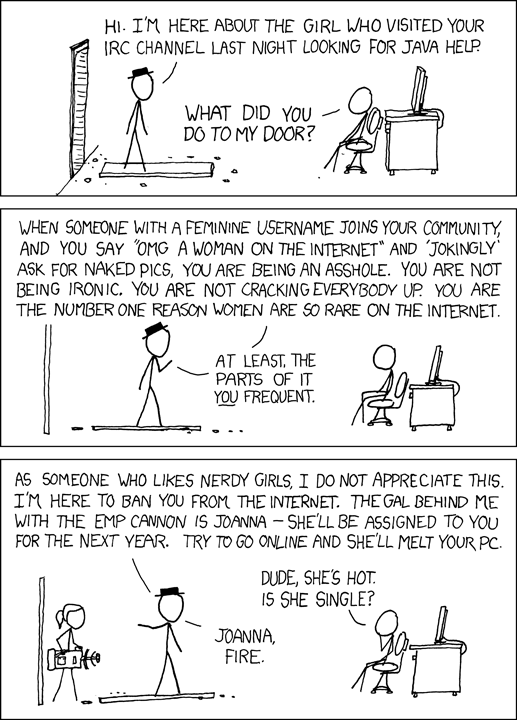
\includegraphics[height=250pt]{pix_plz}
    \end{center}
  \end{figure}
\end{frame}

\end{document}
